\documentclass{article}
\usepackage[utf8]{inputenc}
\usepackage[margin=1in,headheight=24pt]{geometry}
\usepackage{listings}
\usepackage{amsmath}
\usepackage{xcolor}
\allowdisplaybreaks
\usepackage{graphicx}
\graphicspath{ {images/} }

\definecolor{codegreen}{rgb}{0,0.6,0}
\definecolor{codegray}{rgb}{0.5,0.5,0.5}
\definecolor{codepurple}{rgb}{0.58,0,0.82}
\definecolor{backcolour}{rgb}{0.95,0.95,0.92}

\lstdefinestyle{mystyle}{
    backgroundcolor=\color{backcolour},   
    commentstyle=\color{codegreen},
    keywordstyle=\color{magenta},
    numberstyle=\tiny\color{codegray},
    stringstyle=\color{codepurple},
    basicstyle=\ttfamily\footnotesize,
    breakatwhitespace=false,         
    breaklines=true,                 
    captionpos=b,                    
    keepspaces=true,                 
    numbers=left,                    
    numbersep=5pt,                  
    showspaces=false,                
    showstringspaces=false,
    showtabs=false,                  
    tabsize=2
}

\lstset{style=mystyle}

\title{EGEE-2110 Engineering Analysis \\ Homework 1}
\author{Kaitlyn Wiseman}
\date{05 March 2021}

\begin{document}

\maketitle

\newpage

\section{}

Problem 1 was to create the following four matrices:

\begin{align*}
    \textbf{A} = \begin{bmatrix}
    -4 & -3 & 2\\
    4 & 3 & -1\\
    -3 & -2 & 1
    \end{bmatrix} &&
    \textbf{B} = \begin{bmatrix}
    1 & -1 & -3\\
    -1 & 2 & 4\\
    1 & 1 & 1
    \end{bmatrix} &&
    \textbf{C} = \begin{bmatrix}    
    2 & 1 & 3\\
    -1 & 0 & 2\\
    3 & 2 & 1
    \end{bmatrix} &&
    \textbf{D} = \begin{bmatrix}
    0 & 1 & 2\\
    1 & 2 & 0\\
    0 & 2 & 1
    \end{bmatrix}
\end{align*}

The code I used to create the four matrices is

\begin{lstlisting}[language=Matlab]
% Create 4 matrices:
A = [-4 -3  2;
      4  3 -1;
     -3 -2  1];
B = [ 1 -1 -3;
     -1  2  4;
      1  1  1];
C = [ 2  1  3;
     -1  0  2;
      3  2  1];
D = [ 0  1  2;
      1  2  0;
      0  2  1];
\end{lstlisting}

The code successfully created the four matrices in memory.

\section{}

Problem 2 was to show by multiplication that \textbf{B} is not the inverse of \textbf{A}.

If \textbf{B} is the inverse of \textbf{A}, \textbf{AB} should equal the identity matrix.  I used the following code to test whether this was true:

\begin{lstlisting}[language=Matlab]
% Show by multiplication that B is not the inverse of A.
disp(' If B is the inverse of A, AB should equal I:')
A * B 
disp(' =\= I.')
\end{lstlisting}

The result of that multiplication is
\begin{align*}
    \text{ans} = \begin{bmatrix}
    1 & 0 & 2\\
    0 & 1 & -1\\
    0 & 0 & 2
    \end{bmatrix}
\end{align*}
which is not the identity matrix.  Hence, \textbf{B} is not the inverse of \textbf{A}.

\section{}

Problem 3 was to find the actual inverse of \textbf{A} and prove it is the inverse.
If \textbf{A\textsuperscript{$-1$}} truly is the inverse of \textbf{A}, then \textbf{A\textsuperscript{$-1$}A} will be the identity matrix.

To find \textbf{A\textsuperscript{$-1$}}, I used Matlab's inv() function.  To prove \textbf{A\textsuperscript{$-1$}} was indeed the inverse of \textbf{A}, I performed matrix multiplication of the two, and found the result to be the identity matrix.  I used the following code:

\begin{lstlisting}[language=Matlab]
% Find the actual inverse of A and prove it is the inverse.
invA = inv(A)
A * invA 
disp(' = I.')
\end{lstlisting}

The inverse of A was
\begin{align*}
    \textbf{A\textsuperscript{$-1$}} = \begin{bmatrix}
    1 & -1 & -3\\
    -1 & 2 & 4\\
    1 & 1 & 0
    \end{bmatrix}
\end{align*}
and the result of the calculation was the identity matrix, hence proving that \textbf{A\textsuperscript{$-1$}} is indeed the inverse of \textbf{A}.

\section{}

Problem 4 was to compute the point-by-point multiplication of C and D.  In Matlab, to compute point-by-point multiplication (as opposed to matrix multiplication) of the entries of a matrix, you have to precede the operator with a period, i.e. '.*'.  To compute this multiplication, I used the following code: 

\begin{lstlisting}[language=Matlab]
% Compute the point-by-point multiplication of C and D.
C .* D
\end{lstlisting}

The result of this calculation was

\begin{align*}
    \begin{bmatrix}
    0 & 1 & 6\\
    -1 & 0 & 0\\
    0 & 4 & 1
    \end{bmatrix}.
\end{align*}

\section{}

Problem 5 was to find the characteristic polynomials for \textbf{C} and \textbf{D}.  In Matlab, to find the coefficients of the characteristic polynomial of a matrix, you can use the poly() function.  In order to find these coefficients, I used the following code:

\begin{lstlisting}[language=Matlab]
% Find the characteristic polynomials for C and D.
polyC = poly(C)
polyD = poly(D)
\end{lstlisting}

The results of these calculations were
\begin{align*}
    \text{polyC} = \begin{bmatrix}
    1 & -3 & -10 & 7
    \end{bmatrix} && \text{polyD} = \begin{bmatrix}
    1 & -3 & 1 & -3
    \end{bmatrix}.
\end{align*}

Hence, from these calculations, the characteristic polynomial of \textbf{C} is
\begin{align*}
    \lambda^3 -3\lambda^2 -10\lambda +7 = 0,
\end{align*}
and the characteristic polynomial of \textbf{D} is 
\begin{align*}
    \lambda^3 -3\lambda^2 + \lambda -3 = 0
\end{align*}

\section{}

Problem 6 was to find the roots of the polynomials found in Problem 5.  Matlab has a function roots() that accepts a vector containing the coefficients of a polynomial and returns the roots of that polynomial.  So, by plugging in the results of Problem 5 (stored in the variables polyC and polyD), I could easily find the roots.  I used the following code:

\begin{lstlisting}[language=Matlab]
% Find the roots of the polynomials.
roots(polyC)
roots(polyD)
\end{lstlisting}

From these calculations, the roots of the characteristic polynomial for \textbf{C} are
\begin{align*}
    \lambda = 4.743, -2.3952, 0.6109,
\end{align*}
and the roots of the characteristic polynomial for \textbf{D} are
\begin{align*}D
    \lambda = 3, j, -j.
\end{align*}

\section{}

Problem 7 was to show that the determinant $\begin{vmatrix}\textbf{CD}\end{vmatrix}$ is equal to $\begin{vmatrix}\textbf{C}\end{vmatrix}\begin{vmatrix}\textbf{D}\end{vmatrix}$.  In order to do this, I computed both quantities and compared them.  In Matlab, the function det() computes the determinant of the input matrix.  I used the following code to carry out the computations:

\begin{lstlisting}[language=Matlab]
% Show that the determinant |CD| is equal to |C||D|.
det(C * D)
det(C) * det(D)
\end{lstlisting}

The result of both calculations was $-21$.

\section{}

Problem 8 was to first create the following matrix in memory:
\begin{align*}
    \textbf{E} = \begin{bmatrix}
    5 & 3 & -4\\
    6 & -2 & 2\\
    7 & 7 & -9
    \end{bmatrix}.
\end{align*}
Then, the problem required I find the matrix of eigenvectors of \textbf{E} and call it \textbf{P}.  Finally, I showed that \textbf{P\textsuperscript{$-1$}EP} is the diagonalized version of \textbf{E}|the similar matrix containing \textbf{E}'s eigenvalues on its diagonal.  I used the following code to do so:

\begin{lstlisting}[language=Matlab]
% Create the matrix E.
E = [ 5  3 -4;
      6 -2  2;
      7  7 -9]
%   a) Find the matrix containing the eigenvectors of E (call it P).
[P,D] = eigs(E)
%   b) Show that inv(P)EP results in a diagonal matrix which contains the 
%      eigenvalues of E on the main diagonal.
P \ E * P  % I would have used inv(P) * E * P, but it was slightly 
           % inaccurate compared to this
\end{lstlisting}

The result of line $6$ was
\begin{align*}
    \textbf{P} = \begin{bmatrix}
    0.3112 & -0.4627 & 0.0454\\
    -0.4400 & -0.6543 & 0.7711\\
    0.8423 & 0.5982 & 0.6351
    \end{bmatrix} && \textbf{D} = \begin{bmatrix}
    -10.0711 & 0 & 0\\
    0 & 4.0711 & 0\\
    0 & 0 & 0.0000
    \end{bmatrix}
\end{align*}
\textbf{P} is a matrix containing \textbf{E}'s eigenvectors.  \textbf{D} is the diagonal matrix containing \textbf{E}'s eigenvalues on its diagonal, and thus it should match the result of line $9$.  The result of line $9$ was
\begin{align*}
    \begin{bmatrix}
    -10.0711 & 0 & 0\\
    0 & 4.0711 & 0\\
    0 & 0 & 0.0000
    \end{bmatrix},
\end{align*}
which indeed is equal to \textbf{D}.  Hence, \textbf{P\textsuperscript{$-1$}EP} does result in a diagonal matrix which contains the eigenvalues of \textbf{E} on its diagonal.

\section{}

Problem 9 involved plotting the following two functions on the same plot from 0 to 100 in steps of 0.001:
\begin{align*}
    y = e^{-0.05t}\sin(t/2), && z = e^{-0.05t}.
\end{align*}
The x-axis label was "Time", the y-axis label was "Magnitude", the grid was on, and the title was "Exponentially decaying Sine".  I used the following code to implement this:

\begin{lstlisting}[language=Matlab]
%    a) Plot the function y from zero to 100 in steps of 0.001.  Label the 
%       x-axis "Time", and the y-axis "Magnitude".  Display the grid.  Give
%       the plot the title "Exponentially decaying Sine".
t = 0:0.001:100;
y = exp(-0.05*t) .* sin(t/2);

figure(1)
plot(t,y,'linewidth',2)
grid on
xlabel('Time')
ylabel('Magnitude')
title('Exponentially decaying Sine')

hold on

%    b) Plot the function z on the same plot in a different color.  Give
%       the figure a legend, and identify each function with a name ("y"
%       and "z" will work).
z = exp(-0.05*t);

plot(t,z,'linewidth',2,'color','m','linestyle','-.')
legend('y','z')

hold off
\end{lstlisting}
This code produced the following figure:

\begin{figure}[h]
    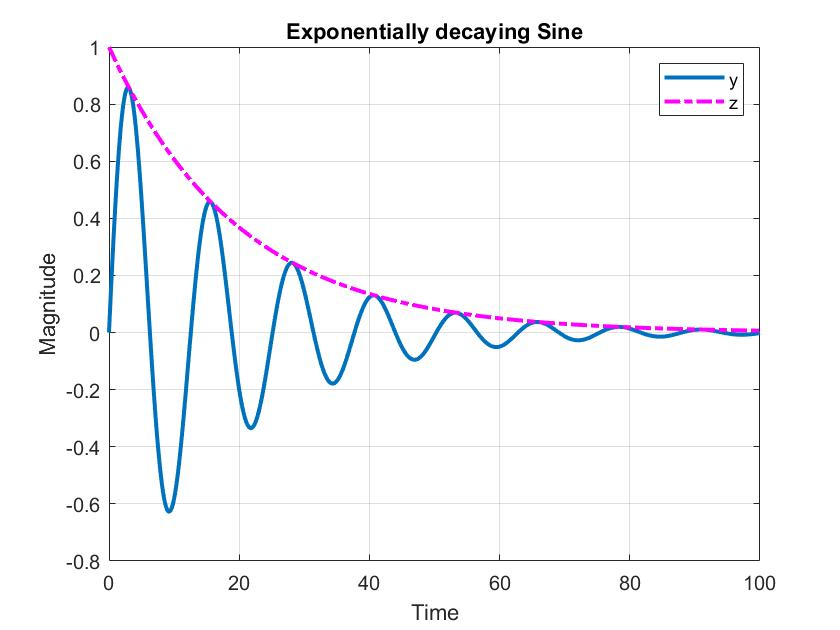
\includegraphics[scale=0.35]{matlab1_9.jpg}
    \centering
\end{figure}

\section{}

Problem 10 was to compute the RMS value of the y function from Problem 9.  To take the RMS value, first square each value, then take the mean of those squares.  Finally, take the square root of the mean.  I used the following code to compute y\textsubscript{RMS}:

\begin{lstlisting}[language=Matlab]
% Compute the RMS value of the signal y from problem 9.  Recall that the 
% name "RMS" tells you the algorithm in reverse order.
yRMS = sqrt(mean(y.^2))
\end{lstlisting}

The result of this calculation was y\textsubscript{RMS} = 0.2225.

\end{document}
